% Figure 1: Delta Accumulator Hardware
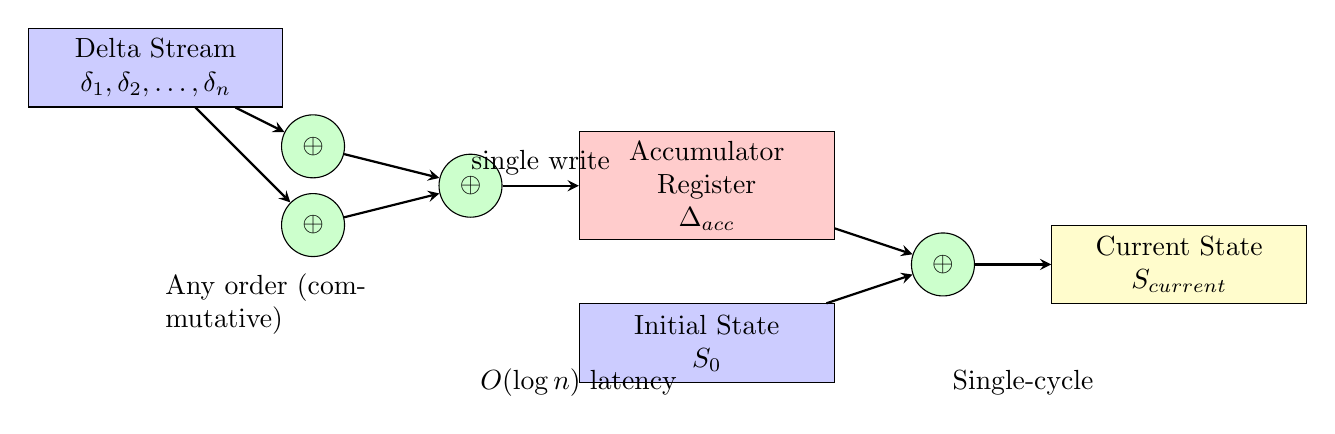
\begin{tikzpicture}[
    block/.style={rectangle, draw, fill=blue!20, text width=3cm, align=center, minimum height=1cm},
    xorgate/.style={circle, draw, fill=green!20, minimum size=0.8cm},
    arrow/.style={->, >=stealth, thick}
]

% Input deltas
\node[block] (input) at (0,4) {Delta Stream\\$\delta_1, \delta_2, \ldots, \delta_n$};

% XOR tree for parallel reduction
\node[xorgate] (xor1) at (2,3) {$\oplus$};
\node[xorgate] (xor2) at (2,2) {$\oplus$};
\node[xorgate] (xor3) at (4,2.5) {$\oplus$};

% Accumulator register
\node[block, fill=red!20] (acc) at (7,2.5) {Accumulator\\Register\\$\Delta_{\text{acc}}$};

% Initial state
\node[block] (init) at (7,0.5) {Initial State\\$S_0$};

% Final XOR for reconstruction
\node[xorgate] (final) at (10,1.5) {$\oplus$};

% Output
\node[block, fill=yellow!20] (output) at (13,1.5) {Current State\\$S_{\text{current}}$};

% Arrows
\draw[arrow] (input) -- (xor1);
\draw[arrow] (input) -- (xor2);
\draw[arrow] (xor1) -- (xor3);
\draw[arrow] (xor2) -- (xor3);
\draw[arrow] (xor3) -- node[above] {single write} (acc);
\draw[arrow] (acc) -- (final);
\draw[arrow] (init) -- (final);
\draw[arrow] (final) -- (output);

% Annotations
\node[anchor=west, text width=3cm] at (0,1) {Any order (commutative)};
\node[anchor=west, text width=3cm] at (4,0) {$O(\log n)$ latency};
\node[anchor=west, text width=3cm] at (10,0) {Single-cycle};

\end{tikzpicture}
